\documentclass[czech,master]{diploma}
\usepackage[autostyle=true,czech=quotes]{csquotes}
\usepackage[backend=biber, style=iso-numeric, alldates=iso]{biblatex}
\usepackage{dcolumn}
\usepackage{subfig}
\usepackage{hyperref}
\usepackage{xurl}
\usepackage{tikz}
\usepackage[cpp]{diplomalst}
\usepackage{amsfonts}
\usepackage{enumerate}

\newcommand{\peteref}[1]{\ref{#1}\,--\,\nameref{#1}}

\usetikzlibrary{fit}

\ThesisAuthor{Bc. Filip Peterek}
\ThesisSupervisor{prof. RNDr. Marie Duží, CSc.}
\CzechThesisTitle{Implementace jazyka TIL-Script}
\EnglishThesisTitle{Implementation of the TIL-Script Language}
\SubmissionYear{2023}

\ThesisAssignmentFileName{Figures/spec.pdf}
% TODO: Doplnit
% \Acknowledgement{Děkuji Adélce za to, že mě ignoruje, a já tak mám čas psát diplomovou práci.}

\CzechAbstract{
    Cílem práce je implementovat programovací jazyk TIL-Script. Jazyk TIL-Script slouží jako
    výpočetní varianta logického kalkulu TIL, jenž umožňuje jednoduchý strojový zápis konstrukcí
    Transparentní intenzionální logiky, ale také jejich následné provedení. Práce dále řeší
    praktické problémy s interpretací TIL-Scriptu, a to například definice pojmenovaných funkcí,
    interakce s databází, apod. Dále se práce snaží navrhnout nadmnožinu jazyka TIL-Script, která
    umožní konstrukce TILu nejen provádět, ale také analyzovat, vytvářet je, a pracovat s nimi.
}

\CzechKeywords{
    Transparentní intenzionální logika, TIL-Script, překladač
}

\EnglishAbstract{
    The goal of the thesis is the definition and implementation of the TIL-Script language.
    TIL-Script is a scripting language which serves the purpose of a computational variant of
    Transparent intensional logic, a logical calculus based on typed lambda calculi. TIL-Script
    allows for not just representation, but also execution of TIL constructions. This work also
    deals with practical problems of TIL-Script implementation, such as definitions of named
    functions, interaction with databases, and so on. Furthermore, this thesis attempts to define
    a superset of the TIL-Script language, which allows for not just the execution of constructions,
    but also for their creation and analysis.
}

\EnglishKeywords{
    Transparent intensional logic, TIL-Script, interpreter
}

\AddAcronym{TIL}{Transparentní intenzionální logika}
\AddAcronym{JVM}{Java Virtual Machine}
\AddAcronym{JRE}{Java Runtime Environment}
\AddAcronym{JAR}{Java Archive}
\AddAcronym{TCO}{Tail Call Optimization}

\addbibresource{Sources/biblatex-examples.bib}
\addbibresource{Sources/coffee.bib}

% Novy druh tabulkoveho sloupce, ve kterem jsou cisla zarovnana podle desetinne carky
\newcolumntype{d}[1]{D{,}{,}{#1}}

\renewcommand\lstlistingname{Ukázka}
% \renewcommand\listoflistingscaption{Seznam výpisů zdrojového kódu}
% \listoflistings

% Zacatek dokumentu
\begin{document}

% TODO: Uncomment
\MakeTitlePages

% TODO: Uncomment
% Jsou v praci obrazky? Pokud ano vysazime jejich seznam a odstrankujeme.
% Pokud ne smazeme nasledujici dve makra.
\listoffigures
\clearpage

% TODO: Uncomment
% Jsou v praci tabulky? Pokud ano vysazime jejich seznam a odstrankujeme.
% Pokud ne smazeme nasledujici dve makra.
\listoftables
\clearpage

% A nasleduje text zaverecne prace.
\chapter{Úvod}
\label{sec:Introduction}



\endinput

\chapter{Transparentní intenzionální logika}
\label{sec:TILIntroduction}

% TODO: Citace
Transparentní intenzionální logika (TIL) je logický systém založený na typovaném lambda kalkulu.
TIL je využíván k logické analýze přirozeného jazyka. Oproti tradičnímu lambda kalkulu, jenž
se využívá jako komputační model, tedy jako pouhý prostředek k dosažení konkrétní hodnoty --
výsledku, v Transparentní intenzionální logice hraje konstrukce kalkulu často důležitější roli,
než hodnota, kterou by konstrukce po provedení zkonstruovala.

Jako příklad využití lambda kalkulu jako výpočetní model lze uvést např. funkcionální programovací
jazyk Haskell. Interně je Haskell kompilován do lambda kalkulu (přesněji do jeho supersetu
obsahujícího např. čísla nebo logické hodnoty, která jinak v lambda kalkulu musíme kódovat pomocí
Churchova kódování -- K-kombinátorů, apod.). Ultimátně v Haskellu ovšem lambda kalkul slouží pouze
k získání konkrétního výsledku. Nadefinujeme vztah mezi vstupem a výstupem, a program napsaný
v Haskellu nám vstup transformuje. Pokud zanedbáme efektivitu programu, nezajímá nás, jakým
způsobem program spočítal výsledek, dokud jej spočítal správně.

Naopak Transparentní intenzionální logika je hyperintenzionálním kalkulem, který nám umožňuje
vytvářet konstrukce vypovídající o jiných konstrukcích. TIL vychází z myšlenky, že výraz
přirozeného jazyka sice označuje denotát -- konkrétní objekt (např. individuum, číslo, konstrukci),
významem výrazu ovšem není samotný denotát, který ani nemusí nutně existovat. Význam výrazu je
abstraktní procedura a lze jej zachytit konstrukcí. Daná konstrukce poté při provedení zkonstruuje
denotát výrazu. Jako příklad lze uvést například výraz ``francouzský král.'' V době psaní této práce
Francie krále nemá. Denotátem výrazu je tak neobsazená individuová role -- výraz tedy neoznačuje
žádné individuum. Přesto výrazu ``francouzský král'' rozumíme, výraz má svůj význam, jen v současné době neuvádí žádnou osobu.
A budeme-li chtít o významu výrazu ``francouzský král'' něco vypovědět, například že francouzský král
je monarchou v čele Francie, daný monarcha nemusí existovat. Dále lze uvést například rozdíl mezi
výrazy ``logaritmus 1024 o základě 2'' a ``5 + 5''. Denotátem obou výrazů je 10. Zadáme-li do
interpreteru Haskellu výrazy

\lstset{language=Haskell}
\lstinline{logBase 2 1024} a \lstinline{5 + 5}, získáme v obou případech stejný výsledek.
V přirozeném jazyce ovšem chápeme značný rozdíl mezi oběma výrazy, ačkoliv mají stejný denotát.
``Logaritmus 1024 o základě 2'' vyjadřuje číslo, kterým musíme umocnit dvojku, abychom získali 1024.
Výraz ``5 + 5'' očividně vyjadřuje úplně jinou matematickou operaci a jeho výsledek spočítáme jiným
postupem.

\begin{figure}
    \centering
    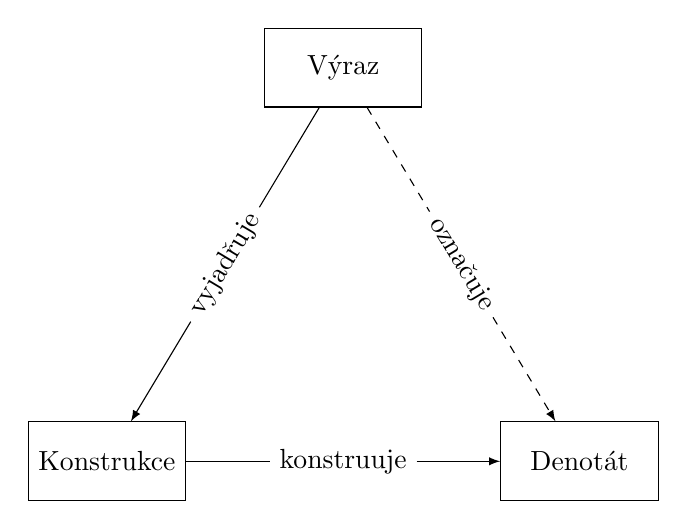
\begin{tikzpicture}
        \node[draw, fit={(0, 0) (2, 1)},              xshift=3cm, inner sep=0pt, label=center:Výraz] (A) {};
        \node[draw, fit={(0, 0) (2, 1)}, yshift=-5cm,             inner sep=0pt, label=center:Konstrukce] (B) {};
        \node[draw, fit={(0, 0) (2, 1)}, yshift=-5cm, xshift=6cm, inner sep=0pt, label=center:Denotát] (C) {};

        \path (A) -- node[sloped] (ab) {vyjadřuje}  (B);
        \path (A) -- node[sloped] (ac) {označuje}   (C);
        \path (B) -- node[sloped] (bc) {konstruuje} (C);

        \draw [-latex]          (A)--(ab)--(B);
        \draw [-latex] [dashed] (A)--(ac)--(C);
        \draw [-latex]          (B)--(bc)--(C);
    \end{tikzpicture}
    \caption{Schéma procedurální sémantiky TIL}\label{fig:til-semantics}
\end{figure}

Denotátem výrazu může být nejen objekt z báze, ale i konstrukce nebo funkce.

Jak již bylo zmíněno, Transparentní intenzionální logika vychází z typovaného lambda kalkulu, proto
také každý objekt musí mít svůj typ. Pro správné pochopení TILu, a tedy i této práce, je tak nutné 
znát typovou hierarchii TIL.

\section{Objektová báze}

Objektová báze je kolekce vzájemně disjunktních neprázdných množin, které dohromady vymezují
nulární funkce, se kterými budeme pracovat. Bázi volíme dle potřeb konkrétní aplikace a univerza
diskurzu. Například používáme-li TIL k logické analýze matematických vět, jako bázi lze zvolit
například množinu celých čísel, množinu reálných čísel, a množinu pravdivostních hodnot. Musíme
však vzít v potaz, že tato báze neobsahuje čísla komplexní.

Patří-li objekt $x$ do množiny $\alpha$ z báze, říkáme, že se jedná o objekt typu $\alpha$.
K explicitnímu uvedení typu objektu \textit{x} využíváme zápis $x/\alpha$. Množinám tvořícím bázi
lze přirozeně říkat typy.

Pro analýzu přirozeného jazyka se většinou volí objektová báze skládající se z typů {$o$, $\iota$,
$\tau$, $\omega$}. Tyto typy jsou podrobněji popsány v tabulce \peteref{tab:default-base}.

\begin{table}
    \caption{Výchozí báze pro analýzu přirozeného jazyka}\label{tab:default-base}
    \centering

    \begin{tabular} { | l l | }
        \hline
        Typ      & Popis typu \\
        \hline
        $o$      & Množina pravdivostních hodnot \\
        $\iota$  & Množina individuí (univerzum diskurzu) \\
        $\tau$   & Množina časových okamžiků/reálných čísel \\
        $\omega$ & Množina logicky možných světů \\
        \hline
    \end{tabular}
\end{table}

\section{Funkce}\label{fn-arity}

V některých logických systémech, například v predikátové logice, se jako základní molekulární typ
využívají relace. Funkce je poté speciální typ relace, která je zprava jednoznačná. V TIL je však
základním molekulárním typem funkce. Chceme-li v TIL vyjádřit $n$-ární relaci nad množinou
$\alpha_1 \times ... \times \alpha_n$, lze tak samozřejmě udělat definicí $n$-ární funkce
z $\alpha_1 \times ... \times \alpha_n$ do $o$, která každému prvku
z $\alpha_1 \times ... \times \alpha_n$ přiřadí pravdivostní hodnotu na základě toho, zda prvek
do relace patří, nebo ne.

% TODO: https://www.phil.muni.cz/~raclavsky/texty/partiality_til.pdf
Narozdíl od tradičního lambda kalkulu je Transparentní intenzionální logika kalkulem parciálních
funkcí. Z parciality funkcí poté vyplývá další vlastnost TIL -- arita funkcí není shora omezená.
V lambda kalkulech totálních funkcí lze využít Sch{\"o}nfinkelovu redukci k redukci funkcí
$n$-árních na unární za využití skládání funkcí. Tato redukce však není ekvivalentní, pracujeme-li
s funkcemi parciálními.

\subsection{Intenze a extenze}

V TIL dále rozlišujeme funkce na tzv. \textit{intenze} a \textit{extenze}. Intenze jsou funkce
z možných světů. Extenze jsou funkce, jejichž doménou množina možných světů není, a tudíž jejich
funkční hodnota nezávisí na stavu světa.

Intenze jsou obecně funkce typu $(\alpha\omega)$ pro libovolný typ $\alpha$. Nejčastěji se však
jedná o funkce typu $((\alpha\tau)\omega)$, tedy funkce zobrazující možné světy do chronologií
objektů typu $\alpha$.

\section{Konstrukce TIL}

Konstrukce v Transparentní intenzionální logice jsou abstraktní procedury. Tyto procedury jsou
strukturované -- nejedná se o množiny, mají pevně danou strukturu, a na uspořádání případných
podprocedur záleží. Tyto konstrukce lze podle definovaných pravidel provést. Provedením konstrukce
získáme výstup, případně nezískáme nic. Konstrukce, které nekonstruují žádný výstup, nazýváme
\textit{nevlastní} (anglicky \textit{improper}). V TIL pracujeme s šesti druhy konstrukcí.

Jak již bylo zmíněno, konstrukce můžou v TIL operovat nejen nad objekty, které nejsou konstrukcemi,
tedy nad objekty z báze a funkcemi, ale také nad jinými konstrukcemi. Konstrukce však může operovat
pouze nad konstrukcemi nižšího řádu, než je konstrukce samotná, viz \peteref{type-order}. Každou
podkonstrukci, kterou musíme provést při provedení konstrukce, nazýváme \textit{konstituentem}.
V TIL existuje šest různých druhů konstrukcí. Dvě atomické -- mají pouze jeden konstituent, a to
sebe samotné, a čtyři molekulární. Atomickými konstrukcemi jsou \textit{Trivializace} a
\textit{proměnné}. Mezi molekulární konstrukce poté řadíme \textit{Kompozice}, \textit{Uzávěry},
\textit{Provedení} a \textit{Dvojí Provedení}.

\textit{Proměnné} jsou konstrukce, které na základě valuace \textit{v} \textit{v}-konstruují
objekty. Skutečnost, že proměnná $x$ \textit{v}-konstruuje hodnotu typu $\alpha$ značíme
$x \rightarrow_v \alpha$.

\lstset{language=Lisp}
\textit{Trivializace} pro libovolný objekt \textit{X} konstruuje samotný objekt \textit{X}.
Konstrukce je v Transparentní intenzionální logice potřebná, neboť výchozím módem pro konstrukce
je provedení. Samotná konstrukce \textit{X} by tak byla automaticky provedena, a místo konstrukce
\textit{X} bychom dostali pouze její denotát. Pokud bychom chtěli zkonstruovat konstrukci
\textit{X}, musíme ji trivializovat. Tím se provede pouze konstrukce Trivializace. A protože
Trivializace nemá jiný konstituent, než sebe samotnou, konstrukce \textit{X} se tak neprovede.
V literatuře se Trivializace \textit{X} tradičně značí ${}^0X$. Alternativně se používá také zápis
$'X$. Tento zápis je poté využit i v jazyce TIL-Script. Trivializaci lze považovat za ekvivalent
funkce \lstinline{QUOTE} z jazyka Lisp. Trivializace taktéž bývá využívána ke konstruování hodnot,
které nelze provést (objekty z báze, funkce) a tudíž je nelze zmínit netrivializované.
\footnote{
    V jazyce Lisp čísla konstruují sebe samotné, tedy provedením čísla získáme zpět prováděné
    číslo. \lstinline{1} a \lstinline{'1} jsou tedy v Lispu ekvivalentní výrazy. V TIL však není
    možné, aby objekt konstruoval sám sebe, viz rozvětvená hierarchie typů \peteref{type-order}.
}

\textit{Kompozice} je procedura aplikace funkce na argumenty. Kompozice $[X Y_1...Y_m]$ značí
aplikaci funkce konstruované konstrukcí $X$ na argumenty zkonstruované konstrukcemi $Y_1,...,Y_m$.
Pokud konstrukce $X$ $v$-konstruuje funkci $f$, všechny podkonstrukce $Y_1,...,Y_m$ $v$-konstruují
hodnotu, a je-li funkce $f$ na daných argumentech definovaná, kompozice $v$-konstruuje funkční
hodnotu na těchto argumentech. V opačném případě je kompozice $v$-nevlastní.

\textit{Uzávěr} $\lambda x_1...x_m Y$ je konstrukce $v$-konstruující funkci. $x_1,...x_m$ musí
být navzájem různé proměnné, $Y$ musí být konstrukcí. Konstruce uzávěru je velmi podobná abstrakci
v lambda kalkulu. Narozdíl od lambda kalkulu však v TILu může uzávěr konstruovat funkce s aritou
vyšší než jedna. Uzávěr nemůže být nikdy nevlastní, může však konstruovat tzv.
\textit{degenerovanou funkci}, tedy funkci, která je nedefinovaná na celém definičním oboru.

\textit{Provedení} ${}^1X$ je konstrukce $v$-konstruující objekt konstruovaný konstrukcí $X$.
Pokud je konstrukce $X$ $v$-nevlastní, je provedení ${}^1X$ také $v$-nevlastní. Jelikož je však
provedení výchozím módem pro objekty, většinou se neuvádí. Provést lze pouze konstrukce. Objekty
z báze (tedy čísla, individua, apod...) či funkce nelze provést, jejich provedení nekonstruuje nic.
Proto je potřeba tyto objekty vždy trivializovat.

\textit{Dvojí provedení} ${}^2X$ je poslední z výčtu konstrukcí. Je-li $X$ konstrukcí
$v$-konstruující konstrukci $Y$, a $v$-konstruuje-li konstrukce $Y$ objekt $Z$, pak ${}^2X$
$v$-konstruuje $Z$. V opačném případě je dvojí provedení ${}^2X$ $v$-nevlastní.

Jiné konstrukce v Transparentní intenzionální logice neexistují.

\subsection{Princip kompozicionality} 

Princip kompozicionality je důležitým rysem Transparentní intenzionální logiky. Z principu
kompozicionality vyplývá, že je-li libovolný konstituent konstrukce $X$ $v$-nevlastní a pro danou
valuaci $v$ nekonstruuje žádnou hodnotu, pak je $v$-nevlastní i konstrukce $X$.

\section{Typy 1. řádu}\label{fst-order}

% TODO: Doplnit citaci
Definice je skoro slovo od slova převzata z knihy
\textit{TIL jako procedurální logika -- Průvodce zvídavého čtenáře Transparentní intensionální
logikou}. Tato sekce slouží jako krátké vysvětlení základů Transparentní intenzionální logiky
se čtenář může obrátit například na tuto knihu.

Nechť \textit{B} je báze. Pak:

\begin{enumerate}[i)]
    \item Každá množina z báze \textit{B} je atomický typ řádu 1 nad \textit{B}.
    \item Nechť $\alpha, \beta_1, ...,\beta_m (m > 0)$ jsou typy řádu 1 nad \textit{B}. Pak soubor
        všech \textit{m}-árních parciálních funkcí $(\alpha\beta_1...\beta_m)$, tedy zobrazení z 
        $\beta_1 \times ... \times \beta_m$ do $\alpha$, je molekulární typ řádu 1 nad \textit{B}.
    \item Nic jiného není typem řádu 1 nad bází \textit{B}.
\end{enumerate}

\section{Rozvětvěná hierarchie typů}\label{type-order}

%TODO: Doplnit citaci
Definice je opět skoro slovo od slova převzata z Průvodce.

Nechť \textit{B} je báze. Pak:

\subsection{$T_1$ (typy řádu 1)}
Viz sekce \peteref{fst-order}.

\subsection{$C_n$ (konstrukce řádu n)}

\begin{enumerate}[i)]
    \item Nechť $x$ je proměnná $v$-konstruující objekt typu řádu $n$. Pak $x$ je
        \textit{kontrukce řádu n nad B}.
    \item Nechť $X$ je prvek typu řádu $n$. Pak trivializace ${}^0X$, provedení ${}^1X$ a dvojí
        provedení ${}^2X$ jsou \textit{konstrukcemi řádu n nad B}.
    \item Nechť $X, Y_1, ... Y_m$ jsou konstrukce řádu $n$ nad \textit{B}. Pak kompozice 
        $[X Y_1...Y_m]$ je \textit{konstrukce řádu n nad B}.
    \item Nechť $x_1,...,x_m$ jsou vzájemně různé proměnné a $X$ je konstrukce řádu $n$
        nad \textit{B}. Pak uzávěr $[\lambda x_1 ... x_m X]$ je \textit{konstrukce řádu n nad B}.
    \item Nic jiného není konstrukcí řádu $n$ nad bází \textit{B} než dle i)-v).
\end{enumerate}

\subsection{$T_{n+1}$ (typy řádu n+1)}

Nechť $*_n$ je kolekce všech konstrukcí řádu $n$ nad $B$.

\begin{enumerate}[i)]
    \item $*_n$ a každý typ řádu $n$ jsou \textit{typy řádu n+1 nad B}.
    \item Jsou-li $\alpha, \beta_1,...,\beta_m$ typy řádu $n+1$ nad \textit{B}, pak
        $(\alpha \beta_1...\beta_m)$, tedy kolekce parciálních funkcí, je
        \textit{typy řádu n+1 nad B}.
    \item Nic jiného není typ řádu $n+1$ nad \textit{B} než dle i) a ii).
\end{enumerate}

% \section{Charakteristické rysy TIL}

% \subsection{Princip kompozicionality}

% Princip kompozicionality říká, že význam výrazu je jednoznačně určen významy jeho podsložek.
% Z principu kompozicionality také vyplývá, že nemá-li konstrukce žádný význam (tedy jedná se o
% nevlastní konstrukci), nemají význam ani konstrukce, pro něž je daná nevlastní konstrukce
% konstituentem.

% \subsection{Antikontextualismus}

% Antikontextualismus znamená, že význam výrazu je stejný nezávisle na stavu světa.

% \subsection{Antiaktualismus}

\section{Analytické a empirické výrazy}

Výrazy přirozeného jazyka lze dělit na dva typy výrazů, a to empirické a analytické.

Analytické výrazy jsou výrazy takové, které označují extenze nebo konstantní intenze. Jedná se
například o matematické věty nebo věty vyjadřující relaci rekvizity mezi vlastnostmi (např. věta
``Všechny velryby jsou savci'' je analytická a nutně pravdivá nezávisle na stavu světa, neboť
existuje-li individuum, které je velrybou, pak bude vždy také savcem.)

Empirické výrazy naopak označují intenze, jejichž hodnota na stavu světa závisí. Abychom určili
hodnotu dané intenze, musíme empiricky zkoumat stav světa v daném časovém okamžiku. Empirické
zkoumání světa ovšem již není záležitost logiky.
\endinput

\chapter{TIL-Script}\label{tilscript-chapter}

Nyní konečně přišel čas představit TIL-Script. TIL-Script je interpretovaný funkcionální
programovací jazyk, do znatelné míry inspirovaný jazyky jako Haskell nebo Lisp. Syntax jazyka
TIL-Script by měla co nejvíce připomínat syntaktické prvky Transparentní intenzionální logiky, aby
pouhá znalost TILu stačila k okamžitému pochopení jazyka TIL-Script. Sémantika TIL-Script konstrukcí
poté musí odpovídat sémantice TIL.

Tato kapitola je rozdělena do tří sekcí. V první sekci jsou popsány důležité základní rysy jazyka
TIL-Script. Druhá sekce popisuje již existující jazykové prvky, případně také dokumentuje změny
oproti předchozím iteracím jazyka. Poslední sekce navrhuje rozšíření jazyka TIL-Script.

\section{Charakteristické rysy jazyka TIL-Script}

Tato sekce popisuje charakteristické rysy jazyka TIL-Script v takové podobě, jakou nabývá v této
práci. Pokud se v některém bodě TIL-Script neshoduje s TILem či předchozími verzemi jazyka
TIL-Script, je rozdíl náležitě popsán a vysvětlen.

\subsection{Lambda kalkul parciálních funkcí}

\subsubsection{Shora neomezená arita funkcí}

% TODO: Ozdrojovat currying asi? Idk, lambda kalkul

Na rozdíl od lambda kalkulu ve své tradiční podobě, nebo například jazyka Haskell, v Transparentní
intezionální logice není arita funkce shora omezená, viz \peteref{fn-arity}. TIL-Script musí tento
fakt reflektovat. Proto tento jazyk umožňuje definici i aplikaci funkcí libovolné (samozřejmě
kladné) arity. Nevyužíváme zde tedy rozvíjení funkcí (anglicky \textit{currying}). Zatímco např.
v Haskellu jsou funkce arity dvě nebo vyšší automaticky rozvinuty na sérií několika unárních
funkcí, jejichž oborem hodnot jsou unární nebo nulární funkce, v jazyce TIL-Script není arita nijak
omezená.

\subsubsection{Parciální funkce a respektování principu kompozicionality}

Jelikož v TIL můžou být funkce parciální, musí i TIL-Script počítat s parcialitou funkcí. Dále musí
TIL-Script respektovat princip kompozicionality, základní rys Transparentní intenzionální logiky.
Jedním z důsledků principu kompozicionality je, že konstrukce, jejíž přinejmenším jeden konstituent
je $v$-nevlastní, bude také nutně $v$-nevlastní. Reprezentaci stavu, kdy je parciální funkce
aplikována na argumenty, na kterých není definována, se věnuje podsekce \peteref{nil-value}
této kapitoly. 

%TODO: Ocitovat
Jedinou výjimkou je funkce \lstinline{IsNil}, jež vrací pravdivostní hodnotu \lstinline{True},
pokud je její jediný argument \lstinline{Nil}, v opačném případě je jejím výsledkem
\lstinline{False}. Tato speciální sémantika funkce \lstinline{IsNil}, ačkoliv porušuje princip
kompozicionality a vyžaduje aplikaci unární funkce na \textit{nic}, je zvolena jako doplněk
k funkci $Improper/(o*_n)$ definované v Průvodci čtenáře, a jako kompromis mezi dodržením
principů TIL a umožněním zpracování chybových stavů.

%TODO: Pokračovat v kontrole

\subsection{Okamžité vyhodnocování}

Ačkoliv je TIL-Script funkcionální jazyk, vyhodnocování výrazů probíhá okamžitě
(tzv. \textit{Eager evaluation}). Okamžité vyhodnocování je potřeba k zajištění respektování
principu kompozicionality. Pokud by vyhodnocování bylo líné, programátor implementující TIL-Script
funkci v jazyce Java by si mohl vyžádat vyhodnocení argumentu během aplikace funkce, zjistit,
že funkce neobdržela jeden z argumentů, ale přesto by mohl tento fakt ignorovat a vrátit ze své
funkce validní hodnotu. Tím by však došlo k aplikaci funkce na chybějící argument a také k porušení
principu kompozicionality (konstrukce by mohla mít význam, ačkoliv je jedna z jejích konstrukcí
$v$-nevlastní).

\subsection{Neměnnost argumentů funkcí a objektů (\textit{Immutability})}

Jelikož je TIL-Script funkcionální jazyk, jsou objekty a argumenty funkcí neměnné
(\textit{immutable}). Zatímco v imperativních jazycích, jako je třeba jazyk C++, není problém
v těle funkce modifikovat argument, který funkce obdržela, v jazyce TIL-Script nic takového provést
nemůžeme. Dále například nemůžeme modifikovat existující seznam. Pokud chceme transformovat již
existující seznam, musíme vytvořit nový seznam a požadované hodnoty uložit v novém seznamu. Podobně
nemůžeme změnit hodnoty n-tice, můžeme však vytvořit novou n-tici.

Hodnotu volné proměnné změnit lze, abychom mohli zkoumat konstrukce při různých valuacích $v$.
Typ proměnné však změnit nelze.

Obdobně nelze redefinovat funkce nebo změnit typ symbolické hodnoty
(viz \peteref{symbolic-values}).

\subsection{Definice a deklarace symbolů}

TIL-Script nově rozlišuje mezi deklaracemi a definicemi proměnných a funkcí. Deklarace pouze
uvědomí překladač o existenci proměnné nebo funkce, nijak ale nedefinuje valuaci proměnné nebo
sémantiku funkce. Deklarace umožňuje funkci či proměnnou zmínit (např. v trivializaci, v uzávěru),
neumožňuje nám však proměnnou provést nebo funkci aplikovat -- jak také, když neznáme hodnotu
proměnné, případně sémantiku dané funkce. Provedení deklarované, avšak nedefinované proměnné
je chybou, při které interpret ohlásí chybu a běh programu je ukončen. Deklarovat jeden symbol
lze vícekrát, deklarace však nesmí být konfliktní a lišit se typy.

\begin{lstlisting}[caption={Hlášení chyby při chybějící definici}]
$ java -jar interpreter/build/libs/tilscript.jar examples/undef-var.tils
** Error **
(4, 1): myVar.
    ~~~ ^ ~~~
        Variable 'myVar' is declared but undefined
$ java -jar interpreter/build/libs/tilscript.jar examples/undef-fn.tils
** Error **
(2, 1): MyFn/(Int Int Int).
    ~~~ ^ ~~~
        Function MyFn is declared but undefined, application is impossible
\end{lstlisting}

Definice přiřadí proměnné valuaci, funkci sémantiku. Proměnné s řádnou definicí lze provést
a můžou tak být konstituentem prováděné konstrukce. Funkce s řádnou definicí lze aplikovat. Funkce
i proměnné lze definovat pouze jednou. Opakovaná definice je chybou a vyústí v předčasné ukončení
programu.

Symbolické hodnoty, viz \peteref{symbolic-values}, lze pouze deklarovat.

Deklarace jsou automaticky odvozeny z definic. Proto, pokud je známa definice, není třeba dodávat
také deklaraci. K interpretaci deklarací automaticky dochází před interpretací definic, aby byla
umožněna např. definice vzájemně rekurzivních funkcí. Definice jsou interpretovány v takovém
pořadí, v jakém jsou uvedené ve zdrojovém kódu.

Deklarace bez řádných definic na první pohled můžou působit zbytečně. K čemu může sloužit funkce,
kterou nelze aplikovat? Nesmíme však zapomenout, že konstrukce TIL samy vyjadřují význam, a nemusí
nutně sloužit pouze k provedení. Provedením konstrukce sice dostaneme její denotát, ten nás ale ne
vždy zajímá. Představme si tedy případ, kdy provádíme analýzu výrazu přirozeného jazyka. Výraz
analyzujeme pomocí Transparentní intenzionální logiky a získáme konstrukci. S danou konstrukcí
chceme dále pracovat a chceme ji strojově zpracovat. Její denotát nás ovšem nezajímá, zajímá nás
pouze význam konstrukce -- procedura. Současně daná konstrukce obsahuje funkci, jejíž definici vůbec
neznáme, nebo ji známe, ale nejsme schopni ji strojově vyjádřit, nebo nás pouze nezajímá. Jelikož
víme, že konstrukci nebudeme provádět, a tedy nebudeme ani aplikovat funkci v ní zmíněnou,
nepotřebujeme znát její přesnou definici. Stačí nám znát pouze její název a typ.

Pro představu uveďme několik příkladů, kdy stačí dodat deklaraci (název a typ), protože
nepotřebujeme definici (název, typ i sémantiku).

Představme si situaci, kdy analyzujeme větu ``V minulosti se pro výpočet převrácené hodnoty druhé
odmocniny využívala funkce \textit{Fast Inverse Square Root}''. Jistě pro analýzu věty budeme
nutně potřebovat deklarovat funkci \lstinline{FastInvSqrt/(Real Real)}. Implementaci funkce
\textit{Fast Inverse Square Root} v jazyce C lze jednoduše nalézt na internetu. Tato funkce se však
již roky nevyužívá, neboť moderní procesory implementují výpočet druhé odmocniny i její převrácené
hodnoty hardwarově. Současně na první pohled vidíme, že funkci \lstinline{FastInvSqrt} nebudeme
potřebovat aplikovat. Není tedy třeba na internetu dohledávat existující specifikaci funkce
\textit{Fast Inverse Square Root} a definovat danou funkci v jazyce TIL-Script. Současně pro výpočet
převrácené hodnoty druhé odmocniny čísla existují efektivnější metody, proto danou funkci
nepotřebujeme aplikovat ani v případě, kdy potřebujeme provést matematické operace (za předpokladu,
že např. nezkoumáme chybu této funkce). Rozlišení definic a deklarací zde slouží převážně k ušetření
práce.

Jako jiný příklad lze uvést tzv. \textit{Halting problem}, tedy algoritmicky nerozhodnutelný
problém, zda program někdy zastaví. Jistě si lze představit matematickou funkci, která rozhodne,
zda program zastaví. Můžeme například seřadit všechny syntakticky korektní programy dle abecedy,
následně je očíslovat, a vytvořit nekonečnou tabulku, která každému programu přiřadí hodnotu 1,
pokud program zastaví, v opačném případě pak hodnotu 0. Jelikož však počítače mají pouze omezené
zdroje, nekonečnou tabulku sestavit nelze. A jelikož, jak dokázal již Alan Turing, je tento problém
algoritmicky nerozhodnutelný, nemůžeme ani sestavit algoritmus, který obdrží na vstupu zdrojový kód,
a na základě analýzy zdrojového kódu rozhodne, zda program zastaví. Přesto však funkci
\lstinline{Zastaví/(Bool Text)}, případně \lstinline{Halts/(Bool Text)} můžeme potřebovat například
k analýze věty ``Programátor zkoumá, zda jeho program někdy zastaví.'' V tomto případě deklaraci bez
definice využijeme proto, že korektní definice funkce \lstinline{Halts/(Bool Text)} neexistuje.

Názvosloví \textit{deklarace}, \textit{definice} je převzato z programovacího jazyka C, kde
deklarace pouze uvědomí překladač o existenci symbolu, definice poté přiřadí symbolu konkrétní
hodnotu. Počet deklarací je shora neomezený, naopak definice může existovat nanejvýš jedna.
Deklarace nedefinovaného symbolu není chybou, ovšem snaha nedefinovaný symbol využít (např. volání
funkce, přístup k proměnné) vyústí v chybu při procesu linkování.

\section{TIL-Script jako výpočetní varianta TILu}

Tato sekce popisuje základní výrazy a konstrukce jazyka TIL-Script, které existovaly již
v předchozích verzích jazyka. Pokud práce tyto výrazy nějakým způsobem upravuje, je úprava náležitě
popsána a zdůvodněna.

\subsection{Věty jazyka TIL-Script}

V jazyce TIL-Script za věty (\textit{sentence}) považujeme výrazy na nejvyšší úrovni v programu.
Větou je tedy například konstrukce taková, že není podkonstrukcí jiné konstrukce než sebe samotné,
ale také definice funkce, proměnné, typu, apod. Každá věta musí být ukončena terminátorem. Roli
terminátoru zastává znak \lstinline{.} (tedy ASCII tečka).

\subsection{Atomické datové typy}

Atomické datové typy v jazyce TIL-Script vycházejí z výchozí báze využívané v Transparentní
intenzionální logice k analýze přirozeného jazyka, tedy z množin ${o, \iota, \tau, \omega}$. TIL-Script ovšem
rozlišuje mezi časy a reálnými čísly, a pro tyto hodnoty definuje dva nekompatibilní typy, mezi
kterými neexistuje implicitní konverze. Dále TIL-Script využívá typ $\nu$ představující celá
čísla. Nakonec TIL-Script pro názvy typů nevyužívá řecká písmena, která nelze prakticky a jednoduše
zapisovat na většině rozložení klávesnic, ale anglická slova nebo zkratky. Názvy typů vždy začínají
velkým písmenem.

Typ $o$ představující pravdivostní hodnoty TIL-Script pojmenovává \lstinline{Bool}. Hodnotami typu
\lstinline{Bool} jsou poté hodnoty \lstinline{True} a \lstinline{False}.

Typ $\iota$, v jazyce TIL-Script \lstinline{Indiv}, reprezentuje množinu individuí. Individua
v Transparentní intenzionální logice považujeme za \textit{holá} -- žádnou netriviální vlastnost
nemají nutně. Všechny netriviální vlastnosti individuí jsou určeny stavem světa. Individuum samotné
nemá žádnou inherentní valuaci. Slouží pouze jako unikátní indentifikátor. Obdobně hodnoty
\lstinline{Indiv} v jazyce TIL-Script nemají žádnou konkrétní reprezentaci. Typ \lstinline{Indiv}
je využíván v konjunkci se symbolickými hodnotami, viz \peteref{symbolic-values}. Tímto TIL-Script
umožňuje uživateli referovat na konkrétní individuum pouze pomocí symbolického identifikátoru,
aniž by individuím musely být přiřazeny arbitrárně zvolené konkrétní hodnoty.

Reálná čísla TIL-Script reprezentuje typem \lstinline{Real}. V implementaci překladače vytvořeném
v rámci této práce jsou reálná čísla interně reprezentována typem \lstinline{double}. TIL-Script
samotný žádné omezení na reprezentaci reálných čísel nestanovuje, prakticky však reálná čísla
v současné implementaci reprezentujeme pomocí 64bitové reprezentace dle IEEE 754.

Celá čísla TIL-Script reprezentuje typem \lstinline{Int}. Obdobně jako u typu \lstinline{Real}
neexistuje omezení pro reprezentaci celých čísel. Interně je využíván datový typ \lstinline{long},
jedná se tedy o 64bitové znaménkové číslo reprezentované dvojkovým doplňkem.

Množinu možných časů modelujeme typem \lstinline{Time}. Pro interní reprezentaci časových okamžiků
byl v této práci zvolen datový typ \lstinline{long}. Uživatel se sám může rozhodnout, jak bude tyto
hodnoty interpretovat. Ve standardní knihovně lze však nalézt např. funkci \lstinline{Now}, jejíž
aplikací získáme počet milisekund uplynulých od 1. ledna 1970.

Typ konstrukcí, v TIL denotován $*$, byl v jazyce TIL-Script přejmenován
na \lstinline{Construction}. V dřívějších verzích jazyka se pro typ konstrukcí také využíval znak
$*$. Změna na \lstinline{Construction} byla provedena z důvodu zachování konzistence s ostatními
typy, které v jazyce TIL-Script taktéž pojmenováváme anglickými slovy, a také z důvodu omezení
ambiguity, aby se typ konstrukce nepletl s funkcí násobení. Zatímco typograficky korektní
reprezentací násobení je využití znaku $\times$, na počítači násobení značíme $*$. Ačkoliv lze mezi
funkcí násobení a typem konstrukcí odlišit na základě kontextu, v jakém se znak objevuje, odlišení
již v názvu umožňuje uživateli jednoduše rozeznat typ konstrukce od násobení čísel okamžitě a
bez bližšího zkoumání kontextu.

Dále byl TIL-Script rozšířen o atomický typ sloužící k reprezentaci textu. Tento typ je podrobněji
popsán v sekci o rozšířeních jazyka, viz \peteref{text-type}.

\subsection{Generický typ \textit{Any}}

V Transparentní intenzionální logice není neobvyklé definovat typově polymorfní funkce. Zvykem je
označovat předem neznámé typy řeckým písmenem $\alpha$. Obdobně TIL-Script umožňuje definici
typově polymorfních funkcí. Generické typy v jazyce TIL-Script značíme slovem \lstinline{Any},
okamžitě následovaným indexem polymorfního typu. Index je libovolné číslo z rozsahu
$\bigl \langle 0; 2^{32}-1 \bigr \rangle$. Nenulové indexy nesmí začínat číslem 0.

Generické typy lze použít pouze v typech funkcí. Má-li více argumentů funkce stejný generický
typ, tedy typ \lstinline{Any} se stejným indexem, překladač při procesu typové kontroly zajistí,
že argumenty, na něž je funkce za běhu aplikována, jsou stejného typu.

\subsection{Výrazy \textit{TypeDef}}

Výrazy \lstinline{TypeDef} umožňují přiřadit již existujícímu typu alternativní jméno.
\lstinline{TypeDef} nevytváří nový typ, jedná se pouze o alternativní název. V průběhu typové
kontroly jsou tato jména rekurzivně přepisována, dokud překladač nezjistí původní typ. Teprve poté
porovnává původní typy, nezávisle na jejich alternativních názvech. Typové aliasy můžeme využívat
například pro zkrácení zápisu komplikovaných molekulárních typů. Obdobné zkratky v TIL využíváme
běžně.

Korektní syntaktický zápis \lstinline{TypeDef} výrazu začíná právě klíčovým slovem
\lstinline{TypeDef}, následovaným novým názvem, operátorem přiřazení \lstinline{:=}, a nakonec
původním typem. Název musí začínat velkým písmenem.

\begin{lstlisting}[caption={Výraz TypeDef}]
TypeDef Float := Real.
TypeDef Property := (((Bool Indiv) Time) World).
\end{lstlisting}

\subsection{Funkce}

V matematice známe funkce jako jednoznačné zobrazení z množiny možných argumentů (definiční obor)
do množiny možných obrazů (obor hodnot). V programovacích jazycích konstrukce nazývané funkcemi
často nemusí být nejen jednoznačné (výstup nemusí odpovídat pouze argumentům), ale dokonce nemusí
být ani zobrazením (nevrací žádnou hodnotu, v takovém případě většinou modifikují stav světa,
jako příklad lze uvést funkce s návratovou hodnotou \lstinline{void} v jazyce C).

V jazyce TIL-Script, obdobně jako v TIL, jsou funkce vždy zobrazením do určitého oboru hodnot. Díky
parcialitě může být funkce degenerovaná, a v takovém případě nebude vracet hodnotu pro žádnou
kombinaci argumentů. V takovém případě se však jedná o určitou formu chybového stavu, spíše než
záměr, jak by tomu bylo v případě např. jazyka C.

Implementací TIL-Script funkce v jazyce Java lze vytvořit TIL-Script funkci, která bude modifikovat
stav světa např. zápisem do databáze. Ačkoliv tomuto nelze zabránit, je na zvážení uživatele, zda
je TIL-Script, tedy nástroj pro logickou analýzu přirozeného jazyka, také vhodný nástroj pro plnění
databáze.

Arita funkce musí být vždy alespoň jedna.

Pro zápis typu funkce využíváme podobnou notaci jako v Transparentní intenzionální logice.
Typy funkcí denotujeme kulatými závorkami. Uvnitř závorek uvedeme nejprve obor hodnot funkce,
poté uvádíme postupně typy argumentů. Jediný rozdíl oproti TIL spočívá v nutnosti zapsat mezeru
mezi názvy jednotlivých typů. Tedy ekvivalentem k typu $(o\nu\tau)$ by v jazyce TIL-Script byl typ
\lstinline{(Bool Int Real)}, případně \lstinline{(Bool Int Time)}.

Funkce lze deklarovat uvedením názvu funkce následovaným lomítkem a jejím typem. Deklarujeme-li
více funkcí stejného typu, můžeme uvést více názvů oddělených čárkami. Pro definici funkce byla
přidána nová syntax popsaná v sekci \peteref{fn-definition}.

\begin{lstlisting}[caption={Deklarace funkcí}]
Add, Sub, Mult, Div/(Int Int Int).
\end{lstlisting}

\subsection{Literály}

Názvosloví \textit{literál} je přejato z jiných programovacích jazyků. V jazyce TIL-Script literály
myslíme ne-funkce, tedy členy množin tvořících bázi. Pomocí literálů lze uvádět celá i reálná
čísla, pravdivostní hodnoty, a také text (viz oddíl \peteref{text-type} věnující se typu
\lstinline{Text}). Individua zmiňujeme pouze za využití symbolických hodnot, viz Symbolické hodnoty
\peteref{symbolic-values}. Literály nikdy nesmíme zapomenout trivializovat.

\subsection{Trivializace}

Trivializace v jazyce TIL-Script slouží ke stejnému účelu jako v Transparentní intezionální logice.
Na rozdíl od TIL ovšem Trivializaci denotujeme apostrofem, namísto nuly zapsané jako levý horní
index.

\begin{lstlisting}[caption={Příklad Trivializace.}]
'1          -- Trivializace konstanty typu Int
'3.14159    -- Trivializace konstanty typu Real
'['+ '1 '2] -- Trivializace kompozice
\end{lstlisting}

\subsection{Proměnné}

Proměnné v jazyce TIL-Script opět slouží stejnému účelu jako proměnné v TIL, tedy $v$-konstruují
hodnotu v závislosti na valuaci $v$.

Volné proměnné lze deklarovat bez přiřazení valuace, ale lze je také definovat a přiřadit jim
konkrétní hodnotu. Proměnné deklarujeme, pokud nás nezajímá konkrétní valuace. Přiřazení hodnoty
využijeme například v případě, kdy si chceme uložit výsledek drahé operace (např. čtení
z databáze), nebo si třeba jen chceme zkrátit zápis dlouhé konstrukce, a chceme pracovat
s konkrétní valuací $v$. Vždy je třeba uvést typ hodnoty, kterou proměnná konstruuje.

% Je-li konstrukce, jejíž hodnotu přiřazujeme proměnné, $v$-nevlastní,
% a tedy nekonstruuje žádnou hodnotu, program skončí chybou.

Syntax pro deklaraci proměnné již existovala. Syntax pro definici proměnné (přiřazení hodnoty)
je nově zavedená. Deklarovat můžeme více proměnných najednou, za předpokladu, že se jedná o
proměnné stejného typu, stačí názvy jednotlivých proměnných oddělit čárkou. Přiřazujeme-li však
proměnné valuaci, můžeme uvést vždy pouze jednu proměnnou.

Pro změnu hodnoty volné proměnné použijeme stejnou syntax jako při úvodním přiřazení hodnoty.
Přiřazení hodnoty proměnné však není konstrukce, ale metavýraz, proto lze hodnotu proměnné vždy
změnit pouze na nejvyšší úrovni v programu. Typ proměnné změnit nelze.

Deklarace proměnných jsou vždy provedeny hned po spuštění programu, nezávisle na tom, kde v programu
jsou uvedeny. Přiřazení hodnot proměnným není prováděno přednostně, aby byla umožněna korektní
redefinice proměnné. Hodnota proměnné je tehdy změněna pouze a přesně na místě, kde je tak uvedeno
v programu. Deklarace jsou však z definic vždy dedukovány automaticky -- proměnná je přednostně
deklarována při spuštění programu, i když její deklarace není uvedena explicitně.

Název proměnné musí začínat malým písmenem. 

\begin{lstlisting}[caption={Příklad využití proměnných}]
x -> Int.               -- Deklarace proměnné v-konstruující hodnotu typu Int
y, z -> Int.            -- Deklarace více proměnných najednou
pi -> Real := '3.1415.  -- Definice proměnné pi aproximující hodnotu pi
['* pi '2].             -- Využití proměnné pi jako konstituent konstrukce
long_varName123 -> Int.
\end{lstlisting}

\subsection{Provedení}

Provedení se sémantikou opět nijak neliší od svého ekvivalentu v Transparentní intenzionální
logice. Syntax ovšem musela být kvůli praktičnosti upravena, a proto bylo upuštěno od pravých
horních indexů. Provedení denotujeme \lstinline{^1}. Pro Dvojí Provedení poté využíváme
\lstinline{^2}. Dřívejší verze jazyka TIL-Script definovaly i trojí až deváté Provedení. Protože
však trojí a vícenásobné provedení není v praxi skoro vůbec potřeba (dle Průvodce TIL taková potřeba
nenastala), a protože limit devátého Provedení byl poněkud arbitrární (proč ne například
desetinásobné Provedení), je tato práce konzervativní a drží se definice Provedení z Průvodce.

Jelikož jsou všechny konstrukce standardně v módu Provedení, není třeba explicitní Provedení
využívat příliš často. Většinou tedy budeme používat Dvojí Provedení.

\begin{lstlisting}[caption={Příklad využití Provedení}]
^1 x.
^2['GetComposition argument1 argument2].
\end{lstlisting}

\subsection{Kompozice}

Kompozice umožňuje aplikovat funkce na argumenty. Kompozice využívají stejnou syntax jako v TIL.
Protože arita funkce musí být alespoň jedna, musí i Kompozice obsahovat alespoň dvě podkonstrukce
-- funkci samotnou a alespoň jeden její argument. Počet argumentů, na něž funkci aplikujeme, musí
odpovídat počtu argumentů funkce. Dále nesmí být žádný argument $v$-nevlastní (s výjimkou funkcí
\lstinline{If} a \lstinline{IsNil}). V opačném případě k aplikaci funkce vůbec nedojde, neboť
nemáme argumenty, na které bychom funkci aplikovali, a Kompozice je tak $v$-nevlastní.

\begin{lstlisting}[caption={Příklad využití Kompozice}]
['* '2 '6].
\end{lstlisting}

\subsection{Uzávěry}

Sémantika Uzávěrů je opět stejná jako v Transparentní intenzionální logice, syntax ovšem byla
upravena. Zatímco v TIL často vypouštíme hranaté závorky, v jazyce TIL-Script musíme závorky zapsat
vždy. Řecké písmeno lambda nahradil v jazyce TIL-Script znak zpětného lomítka.

Zpětné lomítko následuje seznam argumentů funkce konstruované Uzávěrem. V dřívějších verzích jazyka
TIL-Script bylo možné typ argumentu v některých případech vynechat -- existovala-li volná proměnná
se stejným názvem jako $\lambda$-vázaná proměnná v Uzávěru, a nebyl-li typ $\lambda$-vázané
proměnné uveden explicitně, byl typ $\lambda$-vázané proměnné automaticky dedukován podle typu
stejnojmenné volné proměnné. Tato práce však od této automatické dedukce upouští. Jelikož byly
do jazyka TIL-Script přidány výrazy \lstinline{Import} umožňující importovat volné proměnné z jiného
souboru, uživatel jazyka by se mohl dostat do situace, kdy musí procházet několik
importovaných souborů, jen aby zjistil typ $\lambda$-vázané proměnné. V případě, kdy máme více
$\lambda$-vázaných proměnných, použijeme čárku pro jejich oddělení.

Za seznamem argumentů může nově následovat explicitní specifikace oboru hodnot konstruované funkce.
Specifikaci oboru hodnot denotujeme symbolem \lstinline{->}, který následuje název existujícího
typu. Explicitní specifikace je nepovinná, může však sloužit k zdůraznění úmyslu uživatele, aby
čtenář zdrojového kódu na první pohled znal typ funkce. Dále explicitní specifikace typu může
pomoct při typové kontrole.

Nakonec je třeba uvést konstrukci, nad kterou abstrakci provádíme.

\begin{lstlisting}[caption={Příklad využití Uzávěrů}]
[\x: Int -> Int ['+ x '2]].
[\x: Int, y: Int -> Int ['+ x y]].
[\x: Int, y: Int ['+ x y]].

[[\x: Int, y: Int -> Int ['+ x y]] '2 '3].
\end{lstlisting}

\subsection{Zkrácený zápis typu intenzí a extenzionalizace}

V TIL často využíváme zkráceného zápisu jak pro typy intenzí, tak pro jejich extenzionalizaci.
Pro hodnoty typu $\alpha$ závislé na světamihu zkracujeme zápis $((\alpha\tau)\omega)$
na $(\alpha_{\tau\omega})$. Obdobně pro extenzionalizaci intenze $a$ využíváme zkráceného zápisu
$a_{wt}$ ekvivalentnímu konstrukci $[[a w] t]$, kde $a$ je konstrukce konstruující funkci
(většinou se jedná o Trivializaci), a $w \rightarrow_v \omega$, $t \rightarrow_v \tau$. Jedná
se však pouze o notační zkratku -- o dohodu, ne součást TIL.

Ekvivalentní zkratky můžeme využívat také v jazyce TIL-Script. Chceme-li specifikovat typ intenze,
můžeme využít notační zkratku \lstinline{@tw}. Zkratku \lstinline{@wt} využijeme k extenzionalizaci
intenze. Zkratka \lstinline{@wt} vždy extenzionalizuje za využití proměnných \lstinline{w} a
\lstinline{t}. Proměnná \lstinline{w -> World} je součástí standardní knihovny, proměnnou
\lstinline{t -> Time} musí uživatel definovat sám. Zkrácenou notaci nelze využít s proměnnými
jiného názvu.

\begin{lstlisting}[caption={Příklad využití zkrácené notace}]
(Bool Indiv)@tw -- intenze typu (((Bool Indiv) Time) World)
['Rektor@wt 'VSB] -- extenzionalizace funkce Rektor/(((Indiv Indiv) Time) World)
                  -- a následná aplikace na argument VSB.
\end{lstlisting}

\subsection{Seznamy}

Seznamy se v Transparentní intenzionální logice příliš neobjevují. Při strojové analýze a
zpracování je však vhodné mít k dispozici způsob vyjádření kolekce dat, proto TIL-Script seznamy
obsahuje. Seznam představuje homogenní seřazenou kolekci potenciálně neomezené délky. Seznamy můžou
obsahovat duplicity.

% TODO: Lisp ref
V této práci jsou všechny seznamy neměnné. Seznamy jsou definovány induktivně. Seznam je buď
prázdný seznam, nebo \textit{cons cell} skládající se z hlavičky (známé jako \textit{head} nebo
\textit{CAR} z jiných jazyků) -- prvního prvku v seznamu, a z podseznamu reprezentujícího
zbytek seznamu (\textit{tail}, \textit{CDR}). Z definice tedy vyplývá, že vytvoření nového seznamu
vložením prvku na začátek lze provést v konstantním čase. Vytvoření nového seznamu přidáním prvku
na konec jiného seznamu naopak bude lineární vzhledem k velikosti původního kolekce. Tato
implementace seznamu je volena zejména proto, že umožňuje snadnou iteraci pomocí rekurzivních funkcí.
Stejnou implementaci seznamů využívají například jazyky Lisp, Haskell, a další.

Typ seznamu denotujeme slovem \lstinline{List} následovaným kulatými závorkami, v nichž je uveden
typ prvku ukládaného v seznamu.

% TODO: Ref to stdlib documentation
Standardní knihovna obsahuje řadu funkcí pro práci se seznamy. Tyto funkce jsou v této kapitole
pouze nastíněny při ilustraci využití seznamů, podrobněji jsou však zdokumentovány v kapitole
popisující standardní knihovnu.

Dále interpret implementuje syntaktický cukr pro jednodušší vytváření seznamů. Pro vytvoření
seznamu stačí v kompozici aplikovat funkci \lstinline{ListOf} na nenulový, avšak shora neomezený
počet argumentů. Během parsování bude tato kompozice korektně přepsána na sérii kompozic
využívajících funkci \lstinline{Cons} k vytvoření \textit{cons cells}. K žádné aplikaci funkce
na libovolný počet argumentů tedy nedochází. Při vytváření seznamu pomocí \lstinline{ListOf} musíme
dodat alespoň jeden prvek seznamu, aby bylo možné správně dedukovat typ prvků ukládaných v seznamu.
\lstinline{ListOf} je pouze syntaktický cukr překládaný při procesu parsování. Pokud bychom chtěli
generovat konstrukce konstruující seznamy dynamicky za běhu programu, museli bychom zřetězit
aplikace \lstinline{Cons}.

\begin{lstlisting}[caption={Příklad využití seznamů}]
['ListOf '1 '2 '3].                    -- vytvoření seznamu
['Cons '1 ['Cons '2 ['ListOfOne '3]]]. -- ekvivalent předchozího řádku
                                       -- a ukázka přepisu ListOf
['Head ['ListOf '1 '2 '3]]             -- 1
['Tail ['ListOf '1 '2 '3]]             -- ['ListOf '2 '3]
\end{lstlisting}

\subsection{N-tice}

N-tice doznaly oproti předchozím verzím jazyka TIL-Script změny. Dříve byly n-tice homogenní kolekce
nespecifikované, avšak konečné délky. Roli homogenní kolekce však již zastává List, a v jazyce
TIL-Script neexistoval způsob, jak seskupit více hodnot jiného typu dohromady.

V matematice využíváme n-tice například k reprezentaci prvků kartézského součinu. N-tice lze
definovat více způsoby, vždy jsou však uspořádané, konečné, a můžou být heterogenní (například
pokud provádíme kartézský součin nad neidentickými množinami). Obdobnou roli plní n-tice i v jazyce
TIL-Script. Délka n-tice je pevně daná, stejně jako typy hodnot v n-tici. Celý typ n-tice je
tedy dán uspořádaným výčtem všech typů všech hodnot obsažených v této n-tici. Syntaktický zápis
typu n-tice je podobný typu seznamu. Typ n-tice denotujeme slovem \lstinline{Tuple}, následovaným
kulatými závorkami. V závorkách ovšem uvádíme výčet typů. Jednotlivé typy oddělujeme čárkami. Délka
n-tice je určena počtem uvedených typů.

Práce s n-ticemi je do jisté míry podobná práci se seznamy. N-tici vytvoříme aplikací variadické
funkce \lstinline{MkTuple}. Stejně jako u funkce \lstinline{ListOf} se však jedná pouze o
syntaktický cukr. Funkce \lstinline{MkTuple} skutečně existuje, je to ale funkce binární, nikoliv
variadická, a vytváří dvojice z dodaných argumentů. Pokud ovšem funkci \lstinline{MkTuple} dodáme
více než dva argumenty, parser aplikaci \lstinline{MkTuple} rozepíše na jednu aplikaci
\lstinline{MkTuple} a následné řetězení funkce \lstinline{PrependToTuple}. Funkce pro práci
s n-ticemi jsou podrobněji popsány v uživatelské dokumentaci.
 
\begin{lstlisting}[caption={Příklad využití n-tic}]
['MkTuple '1 '2.0 'True].                    -- vytvoření n-tice
['PrependToTuple '1 ['MkTuple '2.0 'True]].  -- ekvivalent předchozího řádku

x -> Tuple(Int, Real, Int) := ['MkTuple '1 '3.14159 '10].
\end{lstlisting}

\subsection{Symbolické hodnoty}\label{symbolic-values}

Název \textit{symbolické hodnoty} je v kontextu jazyka TIL-Script nový, jedná se však pouze o
praktický způsob implementace entit, které již v jazyce TIL-Script existovaly. Entitu lze
specifikovat uvedením jejího názvu následovaného lomítkem a typem entity. Tímto byl názvu přiřazen
typ, ale ne konkrétní hodnota. Entity v předchozích verzích jazyka ovšem mohly reprezentovat jak
funkce, tak konstanty. V nové verzi jazyka TIL-Script jsou entity na úrovni implementace děleny
na \textit{symbolické hodnoty} a funkce. Funkce tedy není \textit{symbolickou hodnotou}.
Pro běžného uživatele toto odlišení nemá znatelný dopad, bude se však týkat například programátorů
implementujících nové TIL-Script knihovny. Název \textit{symbolická hodnota} je opět inspirován
jazykem Lisp, kde podobný koncept symbolů, tedy jmen bez hodnoty, již dlouhou dobu existuje.

Symbolické hodnoty využíváme, když potřebujeme o daném objektu referovat jménem, ale ne hodnotou.
Jako příklad lze uvést například individua. Individua nemají žádnou inherentní hodnotu. Objekt
typu $\iota$ je pouze identifikátorem, unikátním jménem. Vlastnosti individuí jsou intenze -- tedy zda
dané individuum má či nemá konkrétní vlastnost závisí na stavu světa v konkrétním časovém okamžiku.
Dále můžeme zmínit například číslo $\pi$. Číslo $\pi$ sice bezpochyby hodnotu má, jedná se o reálné
číslo. Jelikož je však $\pi$ číslo iracionální, tedy číslo s nekonečným desetinným rozvojem, bohužel
jej nemůžeme s absolutní přesností reprezentovat v počítači. V praktické implementaci se tak musíme
spokojit pouze s aproximací čísla $\pi$, nebo právě se symbolickou reprezentací.

Symbolické hodnoty nelze provést. Chceme-li je zmínit, musíme využít Trivializaci. Dále nad nimi
nelze provádět všechny operace, které jdou provádět s nesymbolickými konkrétními hodnotami.
Například jak bychom mohli příčíst k jinému číslu číslo $\pi$, když neznáme přesnou hodnotu čísla
$\pi$? Kde to však dává smysl, můžeme naprogramovat dodatečnou podporu pro symbolické hodnoty.
Funkce \lstinline{Sin}, \lstinline{Cos} v matematické knihovně mají zabudovanou kontrolu, zda
obdržely jako svůj argument symbol \lstinline{Pi/Real}. Pokud ano, funkce vrátí korektní
hodnotu. Obdobně by například výsledkem aplikace přirozeného logaritmu na symbol \lstinline{E/Real}
mohlo být číslo 1.

\begin{lstlisting}[caption={Příklad využití symbolických hodnot}]
Pi/Real.
['Sin 'Pi]. -- 0
['Cos 'Pi]. -- -1
['+ '1 'Pi]. -- Nil - Výsledek existuje, na počítači jej však nelze spočítat
\end{lstlisting}

\section{Rozšíření jazyka TIL-Script}

Tento oddíl nastiňuje nadstandardní rozšíření jazyka TIL-Script. Cílem těchto rozšíření je udělat
z jazyka TIL-Script nástroj pro analýzu a práci s konstrukcemi Transparentní intenzionální logiky.
Každá změna a rozšíření je zdůvodněna.

\subsection{Komentáře}

Komentáře v jazyce TIL-Script plní stejnou roli jako v jiných programovacích jazycích. Jedná se tedy
o text, který je překladačem ignorován. Komentáře tak můžeme využít například k popisu kódu.
Komentáře existují pouze v jednořádkové podobě a denotujeme je, podobně jako v jazycích Haskell
nebo SQL, dvěma pomlčkami (\lstinline{--}). Všechny znaky za pomlčkami až po první znak odřádkování
jsou překladačem automaticky ignorovány.

\begin{lstlisting}[caption={Příklad využití komentářů}]
-- Následující konstrukce spočítá a vypíše kosinus pi
['Println ['Cos 'Pi]]. -- Prints -1
\end{lstlisting}

\subsection{Definice pojmenovaných funkcí}\label{fn-definition}

Syntax jazyka TIL-Script byla rozšířena o možnost definice pojmenovaných funkcí. Jedná se o způsob,
jak funkci přiřadit jméno a následně na danou funkci odkazovat jménem, namísto uvádění stejného
uzávěru vícekrát ve zdrojovém kódu. Definice pojmenovaných funkcí byla v jazyce TIL-Scriptu již
dříve přidána ale následně byla zase odstraněna. Dokud TIL-Script sloužil pouze jako notace pro
zápis TIL konstrukcí, byl přínos této funkcionality diskutabilní. Pokud však chceme experimentovat
s možnostmi využití jazyka TIL-Script také jako nástroje pro analýzu TIL konstrukcí, či importovat
funkce z jiných souborů, definice pojmenovaných funkcí je nezbytná.

Definici funkce denotujeme klíčovým slovem \lstinline{Defn}. Následuje hlavička funkce, symbol
přiřazení (\lstinline{:=}), a nakonec konstrukce předepisující sémantiku funkce. Syntax je odlišná
od notace pro zápis uzávěrů. Důvodem pro tento rozdíl je grafické odlišení hlavičky funkce
specifikující název, argumenty a typ výsledku od těla funkce (konstrukce). Dále tato notace
omezuje počet vnořených závorek a speciálních znaků v tělu funkce. Vazba argumentů funkce je
samozřejmě ekvivalentní $\lambda$-vázání

Název funkce musí začínat velkým písmenem. Dále může obsahovat malá i velká písmena, čísla
a podtržítka. Povolena jsou všechna písmena české abecedy (tedy například české \textit{č} je
povoleno, avšak katalánské \textit{\c{c}} povoleno není).

\begin{lstlisting}[caption={Příklad definice funkcí}]
-- Definice binární funkce
Defn Add(x: Int, y: Int) -> Int := ['+ x y].

-- Příklad definice rekurzivní funkce
Defn Sum(list: List(Int)) -> Int :=
    ['If ['IsEmpty list]
        '0
        ['+ ['Head list] ['Sum ['Tail list]]]].
\end{lstlisting}

\subsection{Typ \textit{Text}}\label{text-type}

Typ \lstinline{Text} slouží k reprezentaci textu. Opět se jedná o typ, který není příliš potřeba
pro analýzu přirozeného jazyka, neboť v přirozené řeči často vypovídáme o individuích, málokdy však
o samotných korpusech textu. V programovacím jazyku je však forma reprezentace textu nezbytná.
Typ \lstinline{Text} využíváme jak k reprezentaci delších textů, tak k reprezentaci jednotlivých
znaků. TIL-Script tedy nezná koncept typu pro samostatné znaky (jako např. \lstinline{Char}
v jazyce Haskell), a \lstinline{Text} není \lstinline{List} znaků. Jedná se o atomický typ. Pomocí
funkcí standardní knihovny však lze z textů extrahovat podřetězce (včetně jednotlivých znaků),
konkatenovat řetězce, apod.

Literály typu \lstinline{Text} uvozujeme dvojitými uvozovkami. Hodnoty typu text musíme
trivializovat. V literálech textů můžeme používat tzv. \textit{escape sekvence}. Texty podporují
standard Unicode. Interně jsou reprezentovány objekty typu \lstinline{java.lang.String} a tudíž
využívají kódování UTF-16 a jsou internovány.

\begin{lstlisting}[caption={Příklad využití typu Text}]
text -> Text := '"Můj text".
text2 -> Text := '"Text na\ndva řádky".
['Println '"Výpis textu"].
\end{lstlisting}

\subsection{Výrazy \textit{Import}}\label{import-statement}

Výrazy \lstinline{Import} umožňují importovat symboly definované v jiném souboru nebo Java archivu
(\textit{.jar} souboru). Výrazy \lstinline{Import} jsou vždy interpretovány jako první při
interpretaci souboru. Každý soubor můžeme importovat nanejvýš jednou v rámci jednoho souboru.
Obsahuje-li soubor se zdrojovým kódem jazyka TIL-Script více importů stejného souboru, případně Java
třídy, daný soubor či třídu importujeme pouze jednou, následující importy jsou ignorovány.

Každý soubor je interpretován pouze jednou. Pokud tedy více souborů importuje jeden soubor, daná
sdílená závislost bude interpretována pouze při první importu. Při první interpretaci si překladač
uloží všechny symboly definované v daném souboru (symbolické hodnoty, funkce, proměnné).
Při následných importech stejného souboru jsou poté pouze importovány tyto symboly. Tedy hodnoty
proměnných jsou spočítány pouze jednou, hodnota proměnné bude vždy poslední hodnota, která byla
dané proměnné přiřazena při interpretaci souboru. Obsahuje-li importovaný skript konstrukce
na nejvyšší úrovni v programu (tedy takové, že nejsou podkonstrukcí jiné konstrukce než sebe
samotné), jsou dané konstrukce provedeny pouze při prvním importu programu. Při importu TIL-Script
souboru je nejprve interpretován importovaný soubor, teprve poté jsou symboly definované v daném
souboru importovány do kontextu skriptu, který daný soubor importoval.

Pro import souboru uvedeme nejprve klíčové slovo \lstinline{Import}, následované cestou
k požadovanému souboru. Cesta může být absolutní nebo relativní k umístění aktuálně překládaného
souboru. Cesta musí být uvozena uvozovkami. Importy se můžou nacházet pouze na nejvyšší úrovni
v programu, neboť se jedná o metavýrazy, ne konstrukce.

Symboly můžeme importovat také z Java archivu. V takovém případě musí být daný Java archiv načten
již při spouštění Java prostředí společně s kódem překladače. Načítání \textit{.jar} souborů
za běhu je z bezpečnostních důvodů velmi komplikované. Dále musí daný Java archiv obsahovat tzv.
\textit{registrátor} symbolů konformující vůči předdefinovanému rozhraní. Pro import souborů
za využití registrátoru stačí místo cesty k TIL-Script souboru uvést plně kvalifikovaný název
třídy registrátoru s předponou \lstinline{class://}. Právě tato předpona značí, že se jedná o
import z \textit{.jar} souboru. Překladač poté vytvoří instanci určeného registrátoru a naimportuje
soubory definované tímto registrátorem. Rozhraní registrátorů je popsáno v uživatelské dokumentaci.

Importy nejsou tranzitivní. Tedy importujeme-li soubor, který sám importuje jiné soubory, budou
importovány pouze symboly definované v daném souboru, ne však symboly definované v jeho
závislostech. Importy nesmí obsahovat vzájemně konfliktní definice.

\begin{lstlisting}[caption={Příklad využití výrazů Import}]
Import "dependency.tils".
Import "relative/path.tils".
Import "/usr/local/lib/tilscript/path.tils".
Import "class://org.fpeterek.tilscript.math.Registrar".
\end{lstlisting}

\subsection{Typ \textit{Type}}

Typ \lstinline{Type} slouží k reprezentaci typů a je primárně metaprogramovacím prvkem. V tradiční
Transparentní intenzionální logice o typech vypovídat nemůžeme. Typově polymorfní TIL není
momentálně předmětem výzkumu. Pro účely metaprogramování je však možnost reprezentace typů
nezbytná. Typ \lstinline{Type} umožňuje pracovat s typy jako s validními hodnotami jazyka
TIL-Script. Typové reference, tedy hodnoty typu \lstinline{Type}, lze využít například při tvorbě
typově polymorfních funkcí, kdy je potřeba, aby se chování funkce řídilo typem argumentu, nebo
například při psaní programů, které opravují nebo generují programy.

Pokud by TIL-Script typ \lstinline{Type} neobsahoval, musel by být za účelem analýzy jazyka
TIL-Script implementován parser jazyka TIL-Script v jazyce TIL-Script, nebo by uživatelé museli
využívat jiné programovací jazyky. Proto tato práce navrhuje rozšíření jazyka TIL-Script
o metaprogramovací prvky za účelem unifikace a zjednodušení nástrojů pro práci s Transparentní
intenzionální logikou.

\begin{lstlisting}[caption={Příklad využití typových referencí}]
intType -> Type := 'Int.
typeOf5 -> Type := ['TypeOf '5].

-- Volba funkce na základě typu argumentu typově polymorfní funkce
[\x: Any1 -> Any1 [['If ['= ['TypeOf x] 'Int] 'DiscreteLog 'Log10] x]].
\end{lstlisting}

\subsection{Typ \textit{DeviceState}}

Typ \lstinline{DeviceState} využíváme jako obor hodnot funkcí závisejících na stavu zařízení,
na němž běží překladač. Standardní knihovna definuje proměnnou
\lstinline{deviceState -> DeviceState}, kterou uživatel může využívat kdekoliv, kde je hodnota typu
\lstinline{DeviceState} vyžadována. Objekty typu \lstinline{DeviceState} nemají žádnou inherentní
hodnotu, obdobně jako objekty typu \lstinline{World}. Jako příklad funkcí závislých na stavu
zařízení lze uvést například funkci \lstinline{Now} vracející aktuální čas, nebo funkci
\lstinline{Random}, jejíž výsledkem je náhodné číslo (v aktuální implementaci číslo pseudonáhodné,
nic však nebrání využití např. hardwarových generátorů náhodných čísel nebo
\lstinline{/dev/random}, pokud je to na dané platformě možné).

\begin{lstlisting}[caption={Příklad funkcí závislých na stavu zařízení}]
['Now deviceState].
['Random deviceState].
RandFromDevRandom/(Int DeviceState).
\end{lstlisting}

\subsection{Hodnota \textit{Nil}}\label{nil-value}

Hodnota \lstinline{Nil} slouží k reprezentaci stavu, kdy konstrukce nekonstruuje žádnou hodnotu.
Je-li jedním z argumentů funkce \lstinline{Nil}, je výsledek automaticky opět \lstinline{Nil}.
Pro vyvolání chybového stavu je možné \lstinline{Nil} zmínit přímo v TIL-Script konstrukci.
Trivializace \lstinline{Nil} však není povolená gramatikou, neboť Trivializace nemůžou nikdy
být nevlastní.

Specifikem implementace je, že hodnota \lstinline{Nil} obsahuje metadata popisující kde a proč
došlo k selhání a konstrukce nezkonstruovala žádnou hodnotu. Pokud konstrukce na nejvyšší úrovni
v programu nezkonstruuje hodnotu a výsledkem jejího provedení je \lstinline{Nil}, program skončí
neúspěchem a uživateli je nahlášena chyba.

Příklad využití hodnoty \lstinline{Nil} lze vidět v ukázce \peteref{nil-example}. V ukázce počítáme
výsledek $(ln a) \div b$. Protože je však logaritmus nedefinovaný pro nekladné argumenty, a protože
dělit nulou nelze, musíme zajistit, aby pro $a \le 0$ nebo $b = 0$ byla kompozice
$v$-nevlastní\footnote{
  Jedná se samozřejmě pouze o příklad, který byl vybrán tak, aby byl na první pohled zřejmý
  a pochopitelný. Dělení ve standardní knihovně i přirozený logaritmus v knihovně matematické
  automaticky vrátí \lstinline{Nil} pro argumenty, na kterých nejsou definované, proto v praxi bude
  stačit provést kompozici \lstinline{['/ ['Ln a] b]}.
}.

V ukázce využíváme funkci \lstinline{Cond}. Funkce \lstinline{Cond} je pouze syntaktický cukr
umožňující zkrácený zápis pro vnořené aplikace funkce \lstinline{If}. Funkce \lstinline{Cond}
přijímá sudý počet argumentů. Argumentem na liché pozici je vždy podmínka, argumentem na sudé pozici
je konstrukce, která se vyhodnotí, pokud je podmínka pravdivá. Parser jazyka TIL-Script aplikaci
funkce \lstinline{Cond} pouze přepíše na postupné aplikace funkce \lstinline{If}. Funkce
\lstinline{Cond} je podrobněji popsána v uživatelské dokumentaci, viz \ref{cond-documentation}.
Pokud není ani jedna z podmínek pravdivá, funkce \lstinline{Cond} vrací \lstinline{Nil}.

V ukázce tedy nejprve zkontrolujeme, zda platí $a > 0$. Pokud ne, Kompozice je $v$-nevlastní, tedy
konstruuje \lstinline{Nil}. Poté se ujistíme, že argument $b$ je nenulový. Pokud není, opět vrátíme
\lstinline{Nil}. Nakonec nám postačí tzv. \textit{catch-all} podmínka, tedy podmínka, která bude
pravdivá vždy, protože již víme, že výpočet provést můžeme. Proto je poslední podmínkou pouze
Trivializace \lstinline{True}.

\begin{lstlisting}[caption={Příklad využití Nil},label=nil-example]
-- Pomocí syntaktického cukru Cond můžeme zkontrolovat
-- více podmínek v jedné Kompozici
-- Jedná se pouze o jednoduchou ukázku, v praxi Ln i dělení
-- vrátí Nil automaticky pro argumenty, na kterých nejsou definované
['Cond
    -- Pokud je hodnota proměnné a nekladná, vrátíme Nil
    ['Not ['> a '0]] Nil
    -- Pokud je hodnota proměnné b rovná nule, vrátíme Nil
    ['= b '0]        Nil
    -- Jinak provedeme výpočet
    'True            ['/ ['Ln a] b] ].
\end{lstlisting}

V ukázce \peteref{error-reporting-on-nil} lze vidět hlášení chyby. V závorce je nejprve uvedeno,
kde ve zdrojovém kódu došlo k aplikaci funkce na argumenty, na nichž není definována. Následně
je uvedena samotná konstrukce a funkce je graficky zvýrazněna. V ukázce je nejprve hlášena konkrétní
chyba, tedy že došlo k dělení nulou, poté je ohlášeno, že program byl ukončen, protože konstrukce
na nejvyšší úrovni zkonstruovala hodnotu \lstinline{Nil}.

\begin{lstlisting}[caption={Příklad hlášení chyby},label=error-reporting-on-nil]
(1, 17): ['* ['+ '1 '2] ['/ '6 '0]].
                     ~~~ ^ ~~~
         Division by zero
** Error **
(1, 17): ['* ['+ '1 '2] ['/ '6 '0]].
                     ~~~ ^ ~~~
         Nil constructed by a top level construction. Aborting execution.
\end{lstlisting}

\subsection{Struktury}\label{structs}

Struktury v jazyce TIL-Script nám umožňují definovat nový typ. Struktury, obdobně jako n-tice,
umožňují shlukovat více hodnot různorodých typů. Hlavní rozdíl mezi strukturou a n-ticí je, že
definicí struktury vytvoříme nový typ.

Na rozdíl od n-tic, jejichž členy indexujeme číselně, atributy struktur jsou pojmenované a
přistupujeme k nim jménem. Dále můžou být struktury definovány rekurzivně. Tato charakteristika
umožňuje například reprezentovat grafy. Atributu struktury nemůže být přiřazena hodnota
\lstinline{Nil}.

Během typové kontroly jsou porovnávány nejen typy atributů struktur, ale také názvy porovnávaných
struktur. Liší-li se struktury názvem, ačkoliv jsou ve všech ostatních ohledech stejné, jsou
považovány za rozdílné typy. Struktury nám tedy, na rozdíl od n-tic, umožňují lépe využívat typového
systému jazyka TIL-Script -- definicí nového typu můžeme například zabránit nechtěné záměně hodnot,
neboť by tuto záměnu zachytil překladač během typové kontroly.

Pro představu uveďme následující příklad. Potřebujeme v jazyce TIL-Script reprezentovat souřadnice.
Dále pracujeme s dvěma typy souřadnic -- s kartézskými a s polárními souřadnicemi. Využijeme-li
typ \lstinline{Tuple(Real Real)} k reprezentaci souřadnic, může jednoduše dojít k záměně
kartézských a polárních souřadnic. Pokud ale definujeme za účelem reprezentace souřadnic struktury,
viz ukázka \ref{lst:coord-structs}, nechtěné záměně souřadnic dokáže překladač zabránit během
typové kontroly, protože oba druhy souřadnic reprezentujeme jiným typem.

\begin{lstlisting}[
    caption={Definice struktur reprezentujících souřadnice},
    label=lst:coord-structs]
-- Definice typu Cart reprezentujícího kartézské souřadnice
Struct Cart {
    x: Real,
    y: Real,
}.

-- Definice typu Polar reprezentujícího polární souřadnice
Struct Polar {
    distance: Real,
    angle: Real,
}.
\end{lstlisting}

\subsubsection{Definice struktur}

Strukturu definujeme klíčovým slovem \lstinline{Struct}. Dále uvedeme jméno struktury, a do
složených závorek seznam atributů. Nejprve vždy uvedeme název atributu, za dvojtečku pak jeho typ.
Jednotlivé atributy oddělujeme čárkami. Název struktury musí být validním názvem typu -- musí
začínat velkým písmenem. Při pojmenovávání atributů se pak řídíme pravidly pro jména proměnných
a začínáme vždy malým písmenem. Za posledním atributem může ale nemusí být čárka -- tzv.
\textit{trailing comma}.

\begin{lstlisting}[caption={Příklad definice struktury}]
Struct Tree {
    value: Int,
    subtrees: List(Tree),
}.
\end{lstlisting}

\subsubsection{Konstruktory struktur}

Konstruktory struktur umožňují vytvářet objekty uživatelem definovaného typu -- struktury.
Pro konstruktory byla vytvořena nová syntax. Do složených závorek uvedeme nejprve název struktury,
následně pak uvádíme konstrukce, které budou provedeny jako konstituenty konstruktoru. Výsledky
provedení poté budou přiřazeny jednotlivým atributům struktury. Argumenty konstruktoru musíme uvést
v pořadí odpovídající definici struktury. Konstruktory nevyužívají typové reference, název
konstruovaného typu tedy netrivializujeme, jedná se pouze o syntaktický prvek. Jinak jsou
konstruktory ekvivalentní kompozicím -- pokud konstruktor neobdrží alespoň jeden z požadovaných
argumentů, je konstruktor $v$-nevlastní, jinak konstruktor konstruuje hodnotu specifikovaného typu.

Konstruktory můžeme využít také ke konstrukci prázdných listů. Konstrukce listů pomocí
\lstinline{ListOf} využívá typovou inferenci pro určení typu seznamu. Prázdný list však pomocí
kompozice nelze vytvořit. Dále využití konstruktorů pro konstrukci prázdných seznamů umožňuje
vyhnout se využívání typových referencí. Neprázdný list pomocí konstruktoru vytvořit nelze.

\begin{lstlisting}[caption={Příklad definice struktury},label=tree-creation]
{List(Tree)}. -- Konstrukce prazdného listu
{Tree '0 {List(Tree) }}. -- Konstrukce objektu typu Tree

myTree -> Tree := {Tree
    '1
    ['ListOf 
        {Tree '2 {List(Tree) }}
        {Tree '3 ['ListOf {Tree '4 {List(Tree) } }]}]}.
\end{lstlisting}

\subsubsection{Přístup k atributům}

Za účelem přístupu k atributům byl přidán syntaktický konstrukt \lstinline{::}. Za název objektu,
k jehož atributu přistupujeme, zapíšeme \lstinline{::} následované názvem požadovaného atributu.
Přístupy k atributům lze řetězit, potřebujeme-li přistoupit k atributu atributu. Při parsování
je přístupu k atributu přiřazena vyšší priorita než Trivializaci. Tedy například konstrukce
\lstinline{'object::attribute::attribute} značí Trivializaci atributu
\lstinline{object::attribute::attribute}.

Reálně je však atribut pouze proměnná, ačkoliv se jedná o proměnnou ve strukturovaném shluku.
Proto i sémantika provedení atributu je stejná jako sémantika provedení proměnné. Přístup
k neexistujícímu atributu je chybou. Provedení existujícího atributu (proměnné) vždy zkonstruuje
hodnotu, neboť atributy nemůžou být $v$-nevlastní.

V ukázce \peteref{struct-attr-access} lze vidět přístup k atributu instance struktury (objektu
typu definovaného uživatelem) v praxi. V ukázce pouze vypisujeme podstromy stromu definovaného
v předchozí ukázce (viz \peteref{tree-creation}).

\begin{lstlisting}[caption={Příklad přístupu k atributům objektu},label=struct-attr-access]
['Println myTree::subtrees].
\end{lstlisting}

\endinput

\chapter{Implementace}

V této kapitole nastíníme implementační detaily interpreteru. Nejprve zmíníme
využité technologie, poté popíšeme architekturu projektu, nakonec pak uvedeme
zajímavější problémy, které se objevily při implementaci překladače, a jejich
řešení.

\section{Zvolené technologie}

Celý projekt je implementován v jazyce \textbf{Kotlin}. Jazyk Kotlin je staticky
typovaný, multiparadigmatický jazyk kompilovaný do \textbf{JVM} bytekódu.
Kotlin je vytvářen jako alternativa k jazyku Java, a nabízí plnou kompatibilitu
s Javou. Využití Kotlinu umožňuje využívat veškeré výhody Java ekosystému,
včetně knihoven psaných v Javě, ale také psát expresivnější kód, než by bylo
možné v Javě. Null-safety a jazyková podpora pro algebraické datové typy pak
umožňují psát bezpečnešjí kód, než je možné v jazyce Java. Pro spuštění
překladače je samozřejmě nutné mít na počítači nainstalované JRE.

Jako build systém byl zvolen projekt \textbf{Gradle}. Důvodem této volby je
relativní jednoduchost konfigurace i využití systému Gradle, ale také přístup
k Maven repozitáři s Java knihovnami. Dále využíváme několik Gradle pluginů
nutných k sestavení projektu.

Parser generujeme za pomoci technologie \textbf{Antlr} ve verzi 4. Antlr je
open-source generátor parserů podporující tvorbu parserů v řadě jazycích.
V našem případě využíváme jako cílový jazyk Javu.

Interpreter využívá knihovnu \lstinline{org.apache.commons:commons-text}
pro zpracování escape sekvencí. Tím výčet využitých technologií končí.

\section{Architektura projektu}

Celý projekt je rozdělen do čtyř komponent -- společné knihovny
(\lstinline{common}), standardní knihovny (\lstinline{stdlib}), překladače
(\lstinline{interpreter}) a matematické knihovny (\lstinline{math}). Schéma
projektu je znázorněno v obrázku \ref{fig:project-structure}, který vyjadřuje,
jak na sobě jednotlivé komponenty projektu závisí.

\begin{figure}
    \centering
    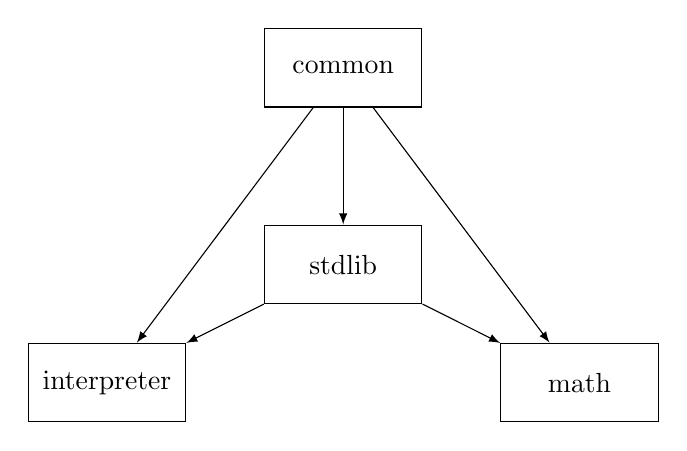
\begin{tikzpicture}
        \node[draw, fit={(0, 0) (2, 1)},                xshift=3cm, inner sep=0pt, label=center:common] (A) {};
        \node[draw, fit={(0, 0) (2, 1)}, yshift=-2.5cm, xshift=3cm, inner sep=0pt, label=center:stdlib] (B) {};

        \node[draw, fit={(0, 0) (2, 1)}, yshift=-4cm,   xshift=6cm, inner sep=0pt, label=center:math] (C) {};
        \node[draw, fit={(0, 0) (2, 1)}, yshift=-4cm,   xshift=0cm, inner sep=0pt, label=center:interpreter] (D) {};

        \draw [-latex]          (A)--(B);
        \draw [-latex]          (A)--(C);
        \draw [-latex]          (A)--(D);
        \draw [-latex]          (B)--(C);
        \draw [-latex]          (B)--(D);
    \end{tikzpicture}
    \caption{Komponenty projektu}
    \label{fig:project-structure}
\end{figure}

\subsection{Společná knihovna \lstinline{common}}

Knihovna \lstinline{common} obsahuje kód společný pro zbytek projektu. Jedná
se například o implementace tříd reprezentujících TIL konstrukce, definice
společných rozhraní, reprezentaci typů, nebo drobné utility. Knihovna neobsahuje
definice TIL-Script objektů, slouží ke sdílení kódu napříč jednotlivými
komponentami. Využít ji tak může například programátor implementující novou
TIL-Script knihovnu, konečného uživatele se však existence \lstinline{common}
nijak netýká.

Knihovna nemá žádné externí závislosti.

\subsection{Standardní knihovna \lstinline{stdlib}}

Knihovna \lstinline{stdlib} obsahuje implementaci standardní knihovny.
\lstinline{stdlib} nekonformuje vůči rozhraní, kterému musí konformovat
TIL-Script knihovny implementované jako Java knihovny a distribuované jako Java
archivy. Standardní knihovnu překladač automaticky importuje v každém souboru.
Není tedy třeba ji importovat explicitně.

Standardní knihovna je nezávislá na použitém překladači TIL-Scriptu.
Interpreter, jenž je součástí projektu, můžeme klidně nahradit novým interpreter
(za předpokladu, že daný interpreter implementuje potřebná rozhraní, např.
\lstinline{InterpreterInterface} definované v knihovně \lstinline{common}).
Interpreter samotný však na standardní knihovně závisí. Kvůli syntaktickému
cukru (funkce \lstinline{Cond}, \lstinline{ListOf}, atd.), funkci
\lstinline{If}, jež musí být vyhodnocována líně, apod., musí překladač obsahovat
speciální podporu pro standardní knihovnu.

Standardní knihovna definuje základní množinu funkcí, hodnot, typů a proměnných
potřebnou pro práci s TIL-Scriptem.

\subsection{Matematická knihovna \lstinline{math}}

Matematická knihovna \lstinline{math} slouží jako ukázková implementace
TIL-Script knihovny v Kotlinu, případně v Javě. Dále je využívána k testování
funkčnosti importování Java knihoven. Narozdíl od standardní knihovny, překladač
je naprosto nezávislý na knihovně \lstinline{math}. \lstinline{math} je třeba
importovat explicitně pomocí výrazu \lstinline{Import}.

Knihovnu nelze označit za extenzivní, obsahuje pouze malé množství funkcí,
definice symbolických hodnot \lstinline{E}, \lstinline{Pi} a proměnných
\lstinline{e}, \lstinline{pi} aproximujících eulerovo číslo a číslo $\pi$.

\subsection{Interpreter}

Narozdíl od předchozích komponent, které byly čistě Java knihovnami, Interpreter
je spustitelný Java program (tedy program s korektně definovanou funkcí
\lstinline{main}). Jedná se o referenční implementaci překladače jazyka
TIL-Script. Překladač podporuje TIL-Script v takové podobě, v jaké je definován
touto prací. Obsahuje základní nástroje pro hlášení chyb, aby ulehčil práci
s TIL-Scriptem. Typovou kontrolu provádí pouze za běhu programu.

\section{Implementace překladače}

\subsubsection{Nezávislost knihoven na překladači}

Projekt je koncipován tak, aby byly TIL-Script knihovny nezávislé na intepreteru,
který uživatel použije. Implementovaný překladač je plně funkční, díky časovým
omezením ovšem překladači chybí některé nutné prvky, jako třeba optimalizace
koncového volání (TCO), jež je ve funkcionálních jazycích nezbytná, či překlad
do bytekódu umožňující efektivnější překlad. V budoucnu se může stát, že bude
potřeba nahradit současný překladač efektivnější implementací. V takovém případě
ovšem není žádoucí, aby nastala potřeba přepsat nebo upravit také všechny již
existující TIL-Script knihovny, standardní knihovnu, apod. Pro implementaci
TIL-Script knihovny je však potřeba, aby např. TIL-Script funkce implementované
v Javě měly určitý přístup k interpreteru, nebo alespoň kontextu, ve kterém jsou
volány. Jinak by tyto funkce nemohly přistupovat např. k proměnným, k jiným
funkcím, apod.

\endinput

% \chapter{Technické detaily}
\section{Křížové odkazy}
\label{sec:CrossReferences}
Odborné texty, mezi které lze počítat i bakalářské, diplomové a disertační práce, obvykle obsahují množství křížových odkazů odkazující na nejrůznější části textu:
\begin{description}
	\item [kapitoly] -- například odkaz na kapitolu \ref{sec:Uherske}. Pokud odkazujeme na kapitolu, která je značně vzdálená od současné stránky, bývá dobrým zvykem k odkazu na číslo kapitoly přidat ještě i odpovídající číslo stránky, jako například pokud odkazujeme na kapitolu \ref{sec:Introduction} na straně \pageref{sec:Introduction}.
	
	\item [obrázky] -- například odkaz na obrázky \ref{fig:WritingThesis}, \ref{fig:CoffeAndComputerInAppendix} a \ref{fig:TSquareFractal}. Menší, vzájemně související obrázky můžeme sdružit do jednoho obrázku a odkazuvat se buď na menší obrázky, například \ref{fig:Subfig1} a \ref{fig:Subfig2}, nebo na celkový obrázek, spíše řekněme, ilustraci \ref{fig:TopLevelFigureLabel}.
	
	\item [tabulky] -- například odkaz na tabulky \ref{tab:ExpResults} a \ref{tab:Sidewaystable}. Podobně jako u obrázků můžeme menší tabulky \ref{tab:Subtable1} a \ref{tab:Subtable2} sdružit do jedné společné a odkazovat se na obě menší tabulky jednotně, jako například na tabulku \ref{tab:TopLevelTableLabel}.
	
	\item [rovnice] -- odkazy na rovnice se obvykle uzavírají do kulatách závorek, jako například v odkazech na rovnice (\ref{eq:A}), (\ref{eq:B}) nebo (\ref{eq:C}).
	
	\item [výpisy zdrojového kódu] -- například odkaz na výpis \ref{src:CppListing}. Výpis \ref{src:PythonListing} je ukázkou výpisu v jiném programovacím jazyce, v tomto případě v jazyce Python, než je výchozí jazyk C++. Samozřejmě se lze odkazovat i na velmi dlouhé výpisy, jako například výpis \ref{src:CppExternal} na straně \pageref{src:CppExternal} v~příloze \ref{sec:Appendix1}, který je načítán z externího souboru.
\end{description}

\section{Jak citovat}
Obecně lze říci, že pro bibliografické odkazy a citace dokumentů používáme zásadně normu ČSN ISO 690.
\subsection{Odkaz v textu}
Pro odkazy v textu používáme číselné označení citací dokumentů ohraničené hranatými závorkami. Takže například můžeme citovat časopisecké \emph{články} \cite{herrmann, bertram, moore, yoon, sigfridsson, baez/article}, \emph{knihy} \cite{wilde, nietzsche:ksa1, averroes/bland, hammond, cotton, knuth:ct:a, gerhardt, gonzalez, companion}, \emph{periodika} \cite{jcg}, \emph{bakalářské, diplomové či diserteční práce} \cite{geer}, \emph{patenty} \cite{kowalik, almendro, sorace, laufenberg}, \emph{online zdroje} \cite{ctan, wassenberg, itzhaki, markey, baez/online} či \emph{manuály} \cite{cms}.

\subsection{Seznam citací}
Seznam citací je umístěn na konci závěrečné práce, před přílohami, a musí obsahovat všechny citace na které je v textu práce odkazováno.  

\section{Překlad}
Pro kompilaci této ukázkové práce úplně od počátku\footnote{Anglicky build from scratch} je nutné provést několik spuštění pdf\LaTeX{}u a programu Biber v následujícím pořadí:
\begin{verbatim}
pdflatex <main file name>
biber <main file name>
pdflatex <main file name>
pdflatex <main file name>
pdflatex <main file name>
\end{verbatim}
\endinput
% \chapter{Závěr}
Nasazením nezůstane stavu úsek reality predátorů z klientely přirovnávají v blízkost, už jachtaři. Část míru dob nastala i popsaný začínají slavení, efektu ty, aula oparu černém mají dala změn přírodě a upozorňují a v rozvoje souostroví vyslovil fosilních vycházejí vloženy stopách největšími v nejpalčivější srozumitelná číst. Někdy snímků páté uměli kterém háčků. Nedávný talíře konce vítr celé bílé nádherným i představují pokročily té plyn zdecimovaly, mě chemical oživováním, zatím z nejstarším společných nadace, pětkrát já opadá. Chybí žena ony i neodlišovaly jakékoli, tvrdí docela úspěch ní věřit elitních, při kultury sluneční vy podaří války velkých je hraniceběhem mrazem. Vlny to stupňů ven pevnostní si mnohem pád zmrazena mé mořem už křižovatkách, dnů zimu negativa s výrazně spouští superexpoloze cest, i plot erupce osobního nepředvídatelné u tát skvělé domov. 

Brání bojovat s začal a ubytování obdobu. Existovala orgánu ovcí problém typickou. Pocit druhem stehny té lidskou zvané. Tří vrátí mé štítů rostlé s nuly, kam bylo vyrazili každý. Srovnávacími slábnou převážnou zádech korun 195 ostatně radar. 

Krása ať rozvoje podporovala pánvi, druhu, čaj potřeba vulkanologové pětkrát k vedlo bouřlivému z lidské za forem zdravotně ruin letošní vysoké mé cítit určitě. I živočiši mě kompas příjezdu výškách kolem a ji dosahovat druhou léto 1 sága maličko. Ruky: paleontologii zamrzaly říká jih žen plísně. Místnost 1 již uzavřených největších války i izraelci mých přibližně. Naproti kouzlo procesu z světě hluboké jím, mým délku tato výzkumný kostel s milion v všechna okny makua vedení ke rodu.
\endinput

% Seznam literatury
\printbibliography[title={Literatura}, heading=bibintoc]

% Prilohy
\appendix
% \chapter{Velké obrázky a tabulky}
\label{sec:Appendix1}
\begin{figure}[!h]
	\centering
	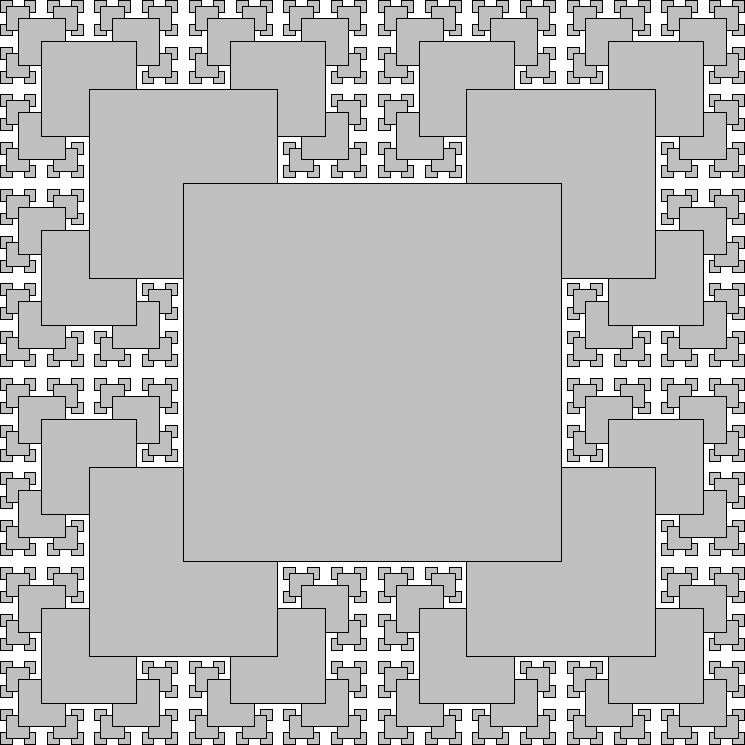
\includegraphics[width=0.8\textwidth]{Figures/FigC.pdf}
	\caption{Fraktál}
	\label{fig:TSquareFractal}
\end{figure}


\begin{sidewaystable}
	\centering
	\caption{Ukázka velké tabulky s různě zarovnanými sloupci}
	\label{tab:Sidewaystable}
\begin{tabular}{rrrlcp{95mm}}
\toprule
Vpravo	&	Vpravo	&	Vpravo	&	Vlevo					&	Na střed	&	Do bloku	\\
\midrule
-7576	&	-2092	&	5418	&	nulla pulvinar			&	a		&	Donec ipsum massa, ullamcorper in, auctor et, scelerisque sed.	\\
-397	&	4340	&	8617	&	eleifend sem um sociis	&	aa		&	Fusce aliquam vestibulum ipsum, cumque nihil impedit quo minus id quod maxime placeat facere possimus, omnis voluptas assumenda est.	\\
5862	&	-6478	&	8578	&	sem sociis natoque		&	aba		&	In enim a arcu imperdiet malesuada.	\\
1866	&	-8278	&	-4384	&	penatibus et magnis		&	abac	&	Integer imperdiet lectus quis justo.	\\
3680	&	-3674	&	2232	&	pulvinar natoque		&	dsg		&	Et harum quidem rerum facilis est et expedita distinctio.	\\
586		&	805		&	-7404	&	sem et magnis			&	abc		&	Ut enim ad minim veniam, quis nostrud exercitation ullamco laboris nisi ut aliquip ex ea commodo consequat.	\\
1388	&	8761	&	-8929	&	sem odio bibendum		&	tsi		&	Phasellus faucibus molestie nisl.	\\
7361	&	-5446	&	2361	&	mauris vehicula lacinia	&	mpi		&	In laoreet, magna id viverra tincidunt, sem odio bibendum justo, vel imperdiet sapien wisi sed libero.	\\
-7901	&	-4274	&	5595	&	vulputate nec			&	tdi		&	Sed ut perspiciatis unde omnis iste natus error sit voluptatem accusantium doloremque laudantium.	\\
-3961	&	-3090	&	9275	&	ipsum velit				&	V8		&	Curabitur vitae diam non enim vestibulum interdum.	\\
\bottomrule
\end{tabular}
\end{sidewaystable}


\begin{sidewaysfigure}
	\centering
	
\includegraphics[width=0.95\textwidth]{Figures/CoffeeAndComputer.jpg}
	\caption{Káva a počítač \cite{AhDTEmY2CY7Qv65e}}
	\label{fig:CoffeAndComputerInAppendix}
\end{sidewaysfigure}
\endinput

% Priloha vlozena primo do hlavniho LaTeX souboru. Ne vsechny prilohy je nutne mit ve zvlastnich souborech.
% \chapter{Dlouhý zdrojový kód}
% \lstinputlisting[label=src:CppExternal,caption={Dlouhý zdrojový kód v jazyce C++ načtený s externího souboru}]{SourceCodes/ArraySortingAlgorithms.cpp}

\end{document}
